Het Microsoft Management Console (MMC) stamt uit 1997 en gebruikt zogenaamde snap-ins. Deze snap-ins worden gebruikt om bepaalde zaken op een Windows systeem te beheren of te controleren. Ook applicatie kunnen gebruik maken van de MMC API om configuratie items via MMC te laten beheren.

Een snap-in gecombineerd met MMC wordt een Management Saved Console genoemd en heeft de msc extensie.

Om Control panel te openen:
\begin{itemize}
\item Klik op het zoek icoon en zoek op mmc
\item Gebruik de windows-toets + r en run mmc
\end{itemize}

\begin{minipage}[t]{\linewidth}
\raggedright
\adjustbox{valign=t}{%
	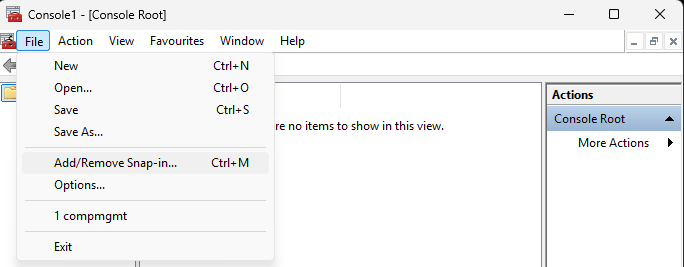
\includegraphics[width=0.99\linewidth]{mmc-snapin.png}%
}
\end{minipage}

Via File kan je snap-ins toevoegen of verwijderen.

We zullen een aantal veel gebruikte snap-ins behandelen in de rest van deze sectie.

